
We train and assess our method using the protein decoy datasets from
the CASP competition \cite{moult2014critical}.  We use the CASP7 to
CASP10 data as training set and the CASP11 data as test set, for a
total of 564 target structures in the training set and 83 target
structures in the test set. Each target from the training set has 282
decoys on average.
%
The test dataset is split into two subsets \cite{kryshtafovych2015}:
``stage 1'' with, for each target, 20 decoys selected at random from
all server predictions from the CASP11 competition, and ``stage 2''
with, for each target, the 150 decoys considered best by the
Davis-QAconsensus evaluation method \cite{kryshtafovych2015}.
%
The native structures were not included in the analysis, neither
during the training phase nor during the testing phase. To make the
structural data more consistent, the side chains of all decoy
structures were optimized using the SCWRL4 program
\cite{krivov2009improved}.


The distributions of target sequences lengths are shown on
Fig. \ref{Fig:dataLengthDist}. They confirm that the two datasets
cover the same range of sequence lengths. To ensure that the training
and test sets are significantly different, we have aligned all test
sequences against all training sequences using blastp
\cite{altschul1990basic}. The most significant alignments (E-value${}
< 10^{-4}$) are shown in Table \ref{Tbl:datasetsSimilarity}.  Less
than 11\% of the targets in the test set (9 out of 83) have sequence
similarity with any target in the training set.

To further assess the evolutionary similarity of the two datasets, we
have computed their overlap in terms of Pfam families
\cite{finn2016pfam}. Pfam families were found using HMMER \cite{hmmer}
with an E-value cutoff of 1.0 \cite{finn2016pfam}.  Table
\ref{Tbl:SharedPfam} shows the targets in the test and train sets that
share a family. Accounting for targets for which no Pfam family could
be determined, approximately 25\% of the test set targets share a
family with approximately 10\% of the training set targets.

We have also compared the structures in the training and test sets
using the ECOD database \cite{cheng2014ecod}. This database provides a
five-level classification of all structures of the RCSB PDB
\cite{berman2000protein} according to the following criteria:
architecture (A-group), possible homology (X-group), homology
(H-group), topology (T-group), and family (F-group).  Since the ECOD
classification is domain-based, multi-domain protein chains can belong
to multiple A-, X-, H-, T-, or F-groups.  The higher the level two
protein domains occupy, the more structurally similar they are.
%
Figure \ref{Fig:foldsGraph} shows the classification of the test set
into ECOD groups. Branches drawn in black correspond to groups
containing structures from the training set as well. Branches drawn in
grey correspond to groups unique to the test set. Targets T0773,
T0797, and T0816 are excluded from the analysis because they have no
ECOD classification, and targets T0820, T0823, T0824, T0827, T0835,
and T0836 are excluded because they have no structure in the RCSB PDB.
%
Four architecture groups present overlap at all levels between the
training and test sets: ``a/b barrels'', ``beta duplicates or obligate
multimers'', ``a+b complex topology'', and ``a+b four layers''.
%%% Is this a useful observation? I don't know what to do with that
%%% information. More generally, I really don't know what to make of
%%% Figure 2. It shows a lot of information that we don't need and the
%%% information we need is mainly in Figure 3.

A more detailed view of the overlap between the training and test sets
is presented in Fig. \ref{Fig:summaryTable}. For each target domain in
the test set (T0759 to T0858), a black tile indicates that at least
one structure from the training set belong to the same ECOD group (A,
X, H, T, and F).
%
%A black tile in the ``Family'' row indicates that at least one
%structure from the training set belongs to the same Pfam family as the
%target. (A grey tile indicates that no Pfam family information is
%available for the target.) A black tile in the ``Clan'' row indicates
%similar information for Pfam clans.
%
%Finally, a black tile in the ``Alignment'' row indicates that at least
%one sequence in the training set aligns to the target sequence with an
%E-value smaller than $10^{-4}$.


\begin{figure}[H]
    \centering
    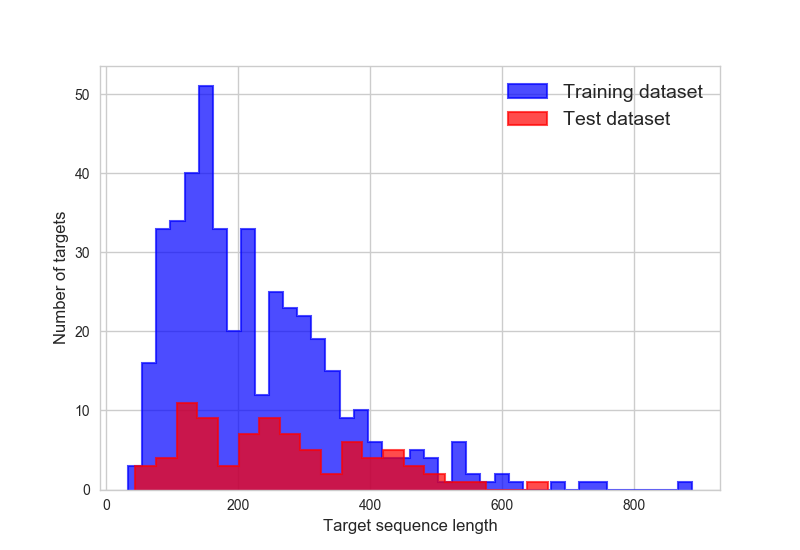
\includegraphics[width=\linewidth]{Fig/datasetLengthDistributions.png}
    \caption{Distributions of sequence lengths for targets in training set (blue) and test set (red).}
    \label{Fig:dataLengthDist}
\end{figure}

\begin{table}[H]
\begin{center}
\begin{tabular}{ c | c | l }
    
    Test set ID & Closest training set ID & E-value \\
    \hline
    T0768 & T0690 & $2.70\times 10^{-13}$ \\
    T0770 & T0645 & $1.79\times 10^{-13}$ \\
    T0772 & T0518 & $1.89\times 10^{-7}$ \\
    T0776 & T0707 & $3.98\times 10^{-5}$ \\
    T0783 & T0699 & $1.19\times 10^{-22}$ \\
    T0798 & T0308 & $9.57\times 10^{-6}$ \\
    T0813 & T0398 & $2.45\times 10^{-5}$ \\
    T0819 & T0636 & $8.66\times 10^{-15}$ \\
    T0854 & T0324 & $2.13\times 10^{-13}$ \\
\end{tabular}
%   
    \caption{Closest homolog sequences from the training set. A
    sequence pair is reported if at least one training sequence aligns
    to a test sequence with a blastp E-value less than $10^{-4}$. Only
    the top alignment is reported for each test sequence.}
%
\label{Tbl:datasetsSimilarity}
\end{center}
\end{table}


\begin{table}[H]
\begin{center}
\begin{tabular}{ l | l | l }

    Common family & Test set target & Train set targets \\
    \hline
    %%% I've removed the version numbers of the Pfam IDs
    %%% I don't think we need them
    PF00795 & T0794 & T0542 \\ \hline
    PF13472 & T0776 & T0448, T0297, T0286, T0750 \\ \hline
    PF03807 & T0813 & T0398, T0393, T0702 \\ \hline
    PF00266 & T0801 & T0339, T0697 \\ \hline
    PF01128 & T0783 & T0699, T0420 \\ \hline
    PF07949 & T0780 & T0572 \\ \hline
    PF13577 & T0815 & T0752, T0736 \\ \hline
    PF12804 & T0783 & T0593, T0699, T0420 \\ \hline
    PF13242 & T0854 & T0371, T0341, T0303, T0324, T0330, T0329, T0418 \\ \hline
    PF13306 & T0768 & T0690, T0671, T0713, T0653 \\ \hline
    PF12741 & T0770 & T0664, T0645, T0532 \\ \hline
    PF00025 & T0798 & T0308 \\ \hline
    PF12872 & T0792 & T0549 \\ \hline
    PF03446 & T0813, T0851 & T0398, T0393, T0702 \\ \hline
    PF00155 & T0801, T0819 & T0591, T0636, T0436, T0697 \\ \hline
    PF13419 & T0854 & T0371, T0341, T0303, T0379, T0324, T0330, T0329, T0418, T0635 \\ \hline
    PF12680 & T0815 & T0451, T0475 \\ \hline
    PF06439 & T0772 & T0518 \\ \hline
    PF12771 & T0770 & T0664, T0645, T0532 \\ \hline
    PF08477 & T0798 & T0308 \\ \hline
    PF00657 & T0776 & T0297, T0286, T0679 \\ \hline
    PF00071 & T0798 & T0308 \\ \hline
    PF00702 & T0854 & T0303, T0324, T0330, T0329, T0418, T0635 \\ \hline
    PF01926 & T0798 & T0308 \\ \hline
    PF12697 & T0764 & T0672 \\ \hline
\end{tabular}
   
\caption{Targets from test and training sets that belong to the same Pfam
family \cite{finn2016pfam}, based on a HMMER search \cite{} with an
E-value cutoff of 1.0. With that cutoff, 403 of the 564 training
targets and 65 of the 83 test targets could be assigned
families. There are 25 families containing at least one test sequence
and one training sequence, involving a total of 16 test targets and 42
training targets. Each of the 25 families belongs to a distinct Pfam
clan.}
%
\label{Tbl:SharedPfam}
\end{center}
\end{table}

\begin{figure}[H]
    \centering
    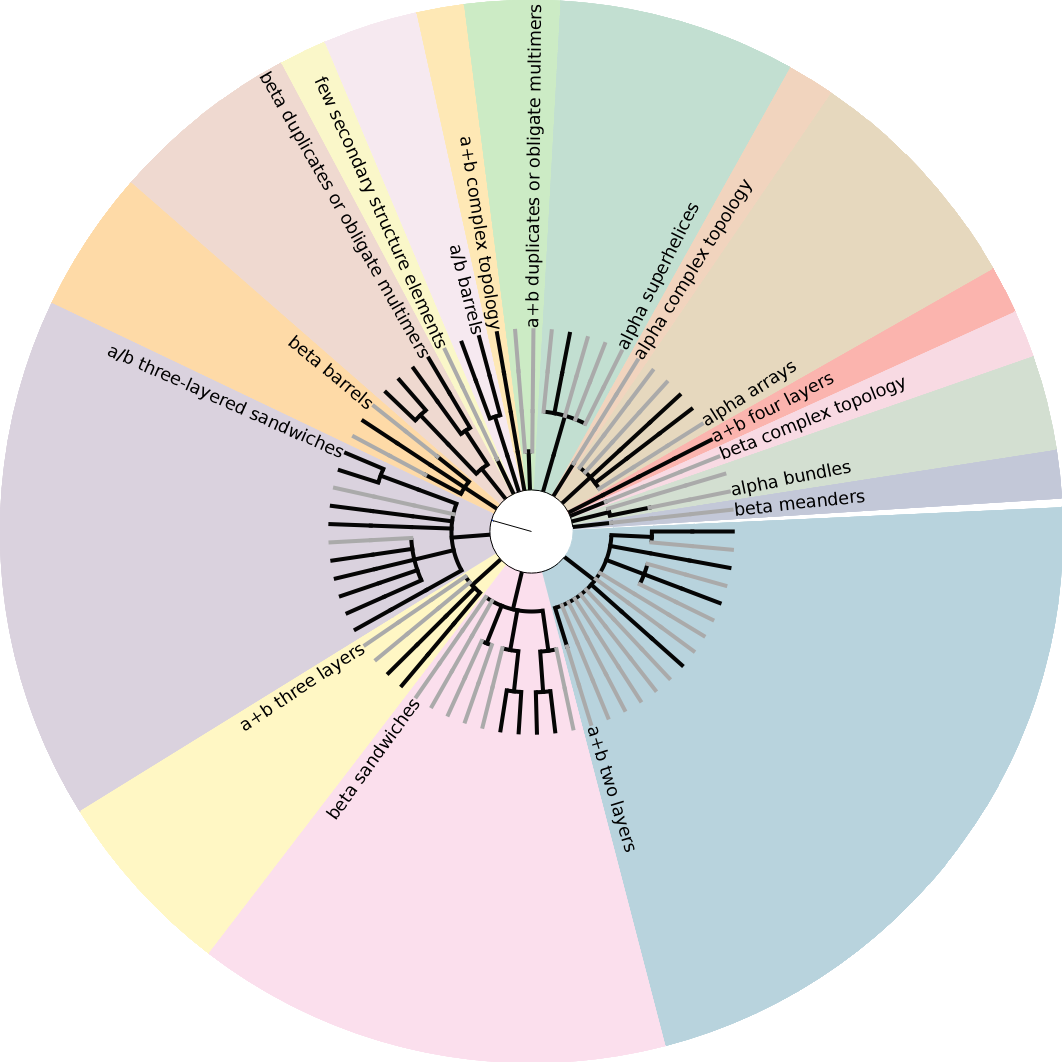
\includegraphics[width=\linewidth]{Fig/folds_graph.png}
%
    \caption{Classification of the test set structures into the lower
    four ECOD structural levels (from the center out): architecture
    (A), possible homology (X), homology (H), and topology (T). The
    names of the architecture types are shown in the outer circle of
    the diagram.
%%% Why do you have two different architecture names in the same A
%%% group? (brown color: ``alpha complex topology'' and ``alpha
%%% arrays'')
    The grey lines denote test set classes that have no
    respective representative in the training set. The black lines
    show the classes that have representatives in both training and
    test sets. We do not show the F-groups because they have litle
    overlap among the training and test sets.
%%% Why not showing the F-groups?
}
%
    \label{Fig:foldsGraph}
\end{figure}

\begin{figure}[H]
    \makebox[\textwidth]{
    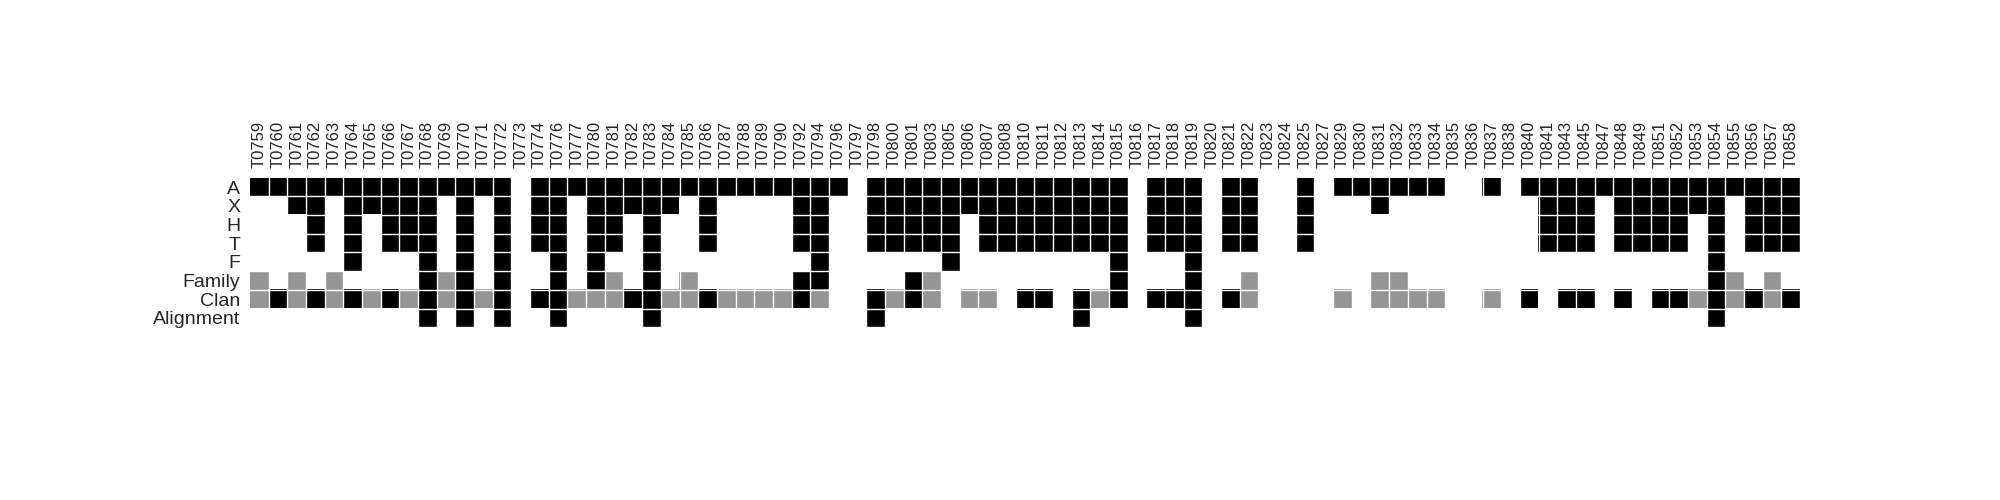
\includegraphics[width=\paperwidth]{Fig/summary_table.png}
    }
%
    \caption{Overlap of the training set on each target domain of the
    test set (from T0759 to T0858). The first 5 rows of tiles
    correspond to the ECOD classification of protein domains (A-, X-,
    H-, T-, and F-groups). A black tile in any of these rows indicates
    that at least one structure from the training set belongs to the
    same ECOD group as the target. Targets for which no ECOD
    classification is available are left empty.
%%% I see that all targets excluded from the analysis have an empty
%%% row of squares. Is T0838 excluded as well? What about the targets
%%% that are not in the list? (775, 778, 779, 791, 793, 795, 799, 802,
%%% 804, 809, 826, 828, 839, 842, 844, 846, 850) Were they all
%%% excluded from the CASP competition? The CASP11 QA paper mentions
%%% that the following targets were cancelled by the organizers: 778,
%%% 779, 791, 809, 842, 844, 846, 850. What about the other ones?
    A black tile in the ``Family'' row indicates that at least one
    structure from the training set belongs to the same Pfam family as
    the target. (A grey tile indicates that no Pfam family information
    is available for the target.) The ``Clan'' row shows similar
    information for Pfam clans. A black tile in the ``Alignment'' row
    indicates that at least one sequence in the training set aligns to
    the target sequence with an E-value smaller than $10^{-4}$.}
%
    \label{Fig:summaryTable}
\end{figure}
